%
\begin{isabellebody}%
\def\isabellecontext{Interfaces}%
%
\isadelimtheory
%
\endisadelimtheory
%
\isatagtheory
\isacommand{theory}\isamarkupfalse%
\ Interfaces\isanewline
\isakeyword{imports}\ Base\isanewline
\isakeyword{begin}%
\endisatagtheory
{\isafoldtheory}%
%
\isadelimtheory
%
\endisadelimtheory
%
\isamarkupchapter{User interfaces%
}
\isamarkuptrue%
%
\isamarkupsection{Isabelle/jEdit Prover IDE \label{sec:tool-jedit}%
}
\isamarkuptrue%
%
\begin{isamarkuptext}%
The \indexdef{}{tool}{jedit}\hypertarget{tool.jedit}{\hyperlink{tool.jedit}{\mbox{\isa{\isatool{jedit}}}}} tool invokes a version of jEdit that has
  been augmented with some components to provide a fully-featured
  Prover IDE (based on Isabelle/Scala):
\begin{ttbox}
Usage: isabelle jedit [OPTIONS] [FILES ...]

  Options are:
    -J OPTION    add JVM runtime option (default JEDIT_JAVA_OPTIONS)
    -b           build only
    -d           enable debugger
    -f           fresh build
    -j OPTION    add jEdit runtime option (default JEDIT_OPTIONS)
    -l NAME      logic image name (default ISABELLE_LOGIC)
    -m MODE      add print mode for output

Start jEdit with Isabelle plugin setup and opens theory FILES
(default Scratch.thy).
\end{ttbox}

  The \verb|-l| option specifies the logic image.  The
  \verb|-m| option specifies additional print modes.

  The \verb|-J| and \verb|-j| options allow to pass
  additional low-level options to the JVM or jEdit, respectively.  The
  defaults are provided by the Isabelle settings environment.

  The \verb|-d| option allows to connect to the runtime
  debugger of the JVM.  Note that the Scala Console of Isabelle/jEdit
  is more convenient in most practical situations.

  The \verb|-b| and \verb|-f| options control the
  self-build mechanism of Isabelle/jEdit.  This is only relevant for
  building from sources, which also requires an auxiliary \verb|jedit_build| component.  Official Isabelle releases already include
  a version of Isabelle/jEdit that is built properly.%
\end{isamarkuptext}%
\isamarkuptrue%
%
\isamarkupsection{Proof General / Emacs%
}
\isamarkuptrue%
%
\begin{isamarkuptext}%
The \indexdef{}{tool}{emacs}\hypertarget{tool.emacs}{\hyperlink{tool.emacs}{\mbox{\isa{\isatool{emacs}}}}} tool invokes a version of Emacs and
  Proof General \cite{proofgeneral} within the regular Isabelle
  settings environment (\secref{sec:settings}).  This is more
  convenient than starting Emacs separately, loading the Proof General
  lisp files, and then attempting to start Isabelle with dynamic
  \hyperlink{setting.PATH}{\mbox{\isa{\isatt{PATH}}}} lookup etc.

  The actual interface script is part of the Proof General
  distribution; its usage depends on the particular version.  There
  are some options available, such as \verb|-l| for passing the
  logic image to be used by default, or \verb|-m| to tune the
  standard print mode.  The following Isabelle settings are
  particularly important for Proof General:

  \begin{description}

  \item[\indexdef{}{setting}{PROOFGENERAL\_HOME}\hypertarget{setting.PROOFGENERAL-HOME}{\hyperlink{setting.PROOFGENERAL-HOME}{\mbox{\isa{\isatt{PROOFGENERAL{\isaliteral{5F}{\isacharunderscore}}HOME}}}}}] points to the main
  installation directory of the Proof General distribution.  This is
  implicitly provided for versions of Proof General that are
  distributed as Isabelle component, see also \secref{sec:components};
  otherwise it needs to be configured manually.

  \item[\indexdef{}{setting}{PROOFGENERAL\_OPTIONS}\hypertarget{setting.PROOFGENERAL-OPTIONS}{\hyperlink{setting.PROOFGENERAL-OPTIONS}{\mbox{\isa{\isatt{PROOFGENERAL{\isaliteral{5F}{\isacharunderscore}}OPTIONS}}}}}] is implicitly prefixed to
  the command line of any invocation of the Proof General \verb|interface| script.  This allows to provide persistent default
  options for the invocation of \texttt{isabelle emacs}.

  \end{description}%
\end{isamarkuptext}%
\isamarkuptrue%
%
\isamarkupsection{Plain TTY interaction \label{sec:tool-tty}%
}
\isamarkuptrue%
%
\begin{isamarkuptext}%
The \indexdef{}{tool}{tty}\hypertarget{tool.tty}{\hyperlink{tool.tty}{\mbox{\isa{\isatool{tty}}}}} tool runs the Isabelle process interactively
  within a plain terminal session:
\begin{ttbox}
Usage: isabelle tty [OPTIONS]

  Options are:
    -l NAME      logic image name (default ISABELLE_LOGIC)
    -m MODE      add print mode for output
    -p NAME      line editor program name (default ISABELLE_LINE_EDITOR)

  Run Isabelle process with plain tty interaction and line editor.
\end{ttbox}

  The \verb|-l| option specifies the logic image.  The
  \verb|-m| option specifies additional print modes.  The
  \verb|-p| option specifies an alternative line editor (such
  as the \indexdef{}{executable}{rlwrap}\hypertarget{executable.rlwrap}{\hyperlink{executable.rlwrap}{\mbox{\isa{\isatt{rlwrap}}}}} wrapper for GNU readline); the
  fall-back is to use raw standard input.

  Regular interaction is via the standard Isabelle/Isar toplevel loop.
  The Isar command \hyperlink{command.exit}{\mbox{\isa{\isacommand{exit}}}} drops out into the bare-bones ML
  system, which is occasionally useful for debugging of the Isar
  infrastructure itself.  Invoking \verb|Isar.loop|~\verb|();|
  in ML will return to the Isar toplevel.%
\end{isamarkuptext}%
\isamarkuptrue%
%
\isamarkupsection{Theory graph browser \label{sec:browse}%
}
\isamarkuptrue%
%
\begin{isamarkuptext}%
The Isabelle graph browser is a general tool for visualizing
  dependency graphs.  Certain nodes of the graph (i.e.\ theories) can
  be grouped together in ``directories'', whose contents may be
  hidden, thus enabling the user to collapse irrelevant portions of
  information.  The browser is written in Java, it can be used both as
  a stand-alone application and as an applet.  Note that the option
  \verb|-g| of \indexref{}{tool}{usedir}\hyperlink{tool.usedir}{\mbox{\isa{\isatool{usedir}}}} creates graph presentations
  in batch mode for inclusion in session documents.%
\end{isamarkuptext}%
\isamarkuptrue%
%
\isamarkupsubsection{Invoking the graph browser%
}
\isamarkuptrue%
%
\begin{isamarkuptext}%
The stand-alone version of the graph browser is wrapped up as
  \indexdef{}{tool}{browser}\hypertarget{tool.browser}{\hyperlink{tool.browser}{\mbox{\isa{\isatool{browser}}}}}:
\begin{ttbox}
Usage: isabelle browser [OPTIONS] [GRAPHFILE]

  Options are:
    -b           Admin/build only
    -c           cleanup -- remove GRAPHFILE after use
    -o FILE      output to FILE (ps, eps, pdf)
\end{ttbox}
  When no filename is specified, the browser automatically changes to
  the directory \hyperlink{setting.ISABELLE-BROWSER-INFO}{\mbox{\isa{\isatt{ISABELLE{\isaliteral{5F}{\isacharunderscore}}BROWSER{\isaliteral{5F}{\isacharunderscore}}INFO}}}}.

  \medskip The \verb|-b| option indicates that this is for
  administrative build only, i.e.\ no browser popup if no files are
  given.

  The \verb|-c| option causes the input file to be removed
  after use.

  The \verb|-o| option indicates batch-mode operation, with the
  output written to the indicated file; note that \verb|pdf|
  produces an \verb|eps| copy as well.

  \medskip The applet version of the browser is part of the standard
  WWW theory presentation, see the link ``theory dependencies'' within
  each session index.%
\end{isamarkuptext}%
\isamarkuptrue%
%
\isamarkupsubsection{Using the graph browser%
}
\isamarkuptrue%
%
\begin{isamarkuptext}%
The browser's main window, which is shown in
  \figref{fig:browserwindow}, consists of two sub-windows.  In the
  left sub-window, the directory tree is displayed. The graph itself
  is displayed in the right sub-window.

  \begin{figure}[ht]
  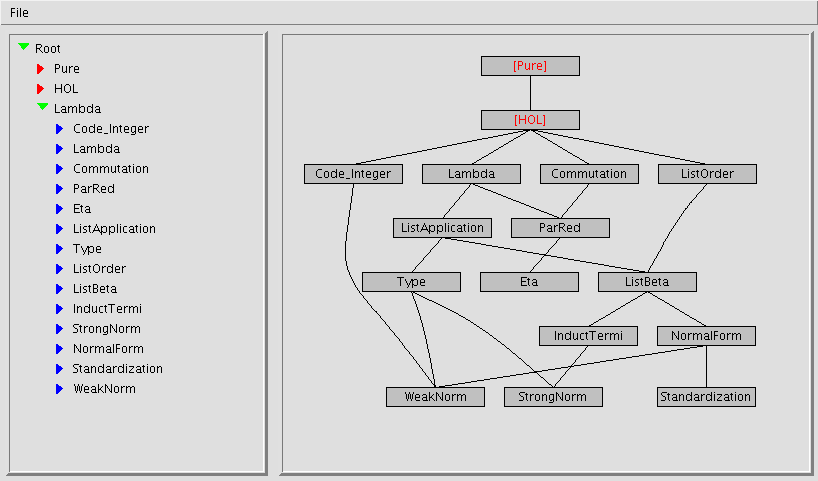
\includegraphics[width=\textwidth]{browser_screenshot}
  \caption{\label{fig:browserwindow} Browser main window}
  \end{figure}%
\end{isamarkuptext}%
\isamarkuptrue%
%
\isamarkupsubsubsection{The directory tree window%
}
\isamarkuptrue%
%
\begin{isamarkuptext}%
We describe the usage of the directory browser and the meaning of
  the different items in the browser window.

  \begin{itemize}

  \item A red arrow before a directory name indicates that the
  directory is currently ``folded'', i.e.~the nodes in this directory
  are collapsed to one single node. In the right sub-window, the names
  of nodes corresponding to folded directories are enclosed in square
  brackets and displayed in red color.

  \item A green downward arrow before a directory name indicates that
  the directory is currently ``unfolded''. It can be folded by
  clicking on the directory name.  Clicking on the name for a second
  time unfolds the directory again.  Alternatively, a directory can
  also be unfolded by clicking on the corresponding node in the right
  sub-window.

  \item Blue arrows stand before ordinary node names. When clicking on
  such a name (i.e.\ that of a theory), the graph display window
  focuses to the corresponding node. Double clicking invokes a text
  viewer window in which the contents of the theory file are
  displayed.

  \end{itemize}%
\end{isamarkuptext}%
\isamarkuptrue%
%
\isamarkupsubsubsection{The graph display window%
}
\isamarkuptrue%
%
\begin{isamarkuptext}%
When pointing on an ordinary node, an upward and a downward arrow is
  shown.  Initially, both of these arrows are green. Clicking on the
  upward or downward arrow collapses all predecessor or successor
  nodes, respectively. The arrow's color then changes to red,
  indicating that the predecessor or successor nodes are currently
  collapsed. The node corresponding to the collapsed nodes has the
  name ``\verb|[....]|''. To uncollapse the nodes again, simply
  click on the red arrow or on the node with the name ``\verb|[....]|''. Similar to the directory browser, the contents of
  theory files can be displayed by double clicking on the
  corresponding node.%
\end{isamarkuptext}%
\isamarkuptrue%
%
\isamarkupsubsubsection{The ``File'' menu%
}
\isamarkuptrue%
%
\begin{isamarkuptext}%
Due to Java Applet security restrictions this menu is only available
  in the full application version. The meaning of the menu items is as
  follows:

  \begin{description}

  \item[Open \dots] Open a new graph file.

  \item[Export to PostScript] Outputs the current graph in Postscript
  format, appropriately scaled to fit on one single sheet of A4 paper.
  The resulting file can be printed directly.

  \item[Export to EPS] Outputs the current graph in Encapsulated
  Postscript format. The resulting file can be included in other
  documents.

  \item[Quit] Quit the graph browser.

  \end{description}%
\end{isamarkuptext}%
\isamarkuptrue%
%
\isamarkupsubsection{Syntax of graph definition files%
}
\isamarkuptrue%
%
\begin{isamarkuptext}%
A graph definition file has the following syntax:

  \begin{center}\small
  \begin{tabular}{rcl}
    \isa{graph} & \isa{{\isaliteral{22}{\isachardoublequote}}{\isaliteral{3D}{\isacharequal}}{\isaliteral{22}{\isachardoublequote}}} & \isa{{\isaliteral{22}{\isachardoublequote}}{\isaliteral{7B}{\isacharbraceleft}}\ vertex{\isaliteral{22}{\isachardoublequote}}}~\verb|;|~\isa{{\isaliteral{22}{\isachardoublequote}}{\isaliteral{7D}{\isacharbraceright}}{\isaliteral{2B}{\isacharplus}}{\isaliteral{22}{\isachardoublequote}}} \\
    \isa{vertex} & \isa{{\isaliteral{22}{\isachardoublequote}}{\isaliteral{3D}{\isacharequal}}{\isaliteral{22}{\isachardoublequote}}} & \isa{{\isaliteral{22}{\isachardoublequote}}vertex{\isaliteral{5F}{\isacharunderscore}}name\ vertex{\isaliteral{5F}{\isacharunderscore}}ID\ dir{\isaliteral{5F}{\isacharunderscore}}name\ {\isaliteral{5B}{\isacharbrackleft}}{\isaliteral{22}{\isachardoublequote}}}~\verb|+|~\isa{{\isaliteral{22}{\isachardoublequote}}{\isaliteral{5D}{\isacharbrackright}}\ path\ {\isaliteral{5B}{\isacharbrackleft}}{\isaliteral{22}{\isachardoublequote}}}~\verb|<|~\isa{{\isaliteral{22}{\isachardoublequote}}{\isaliteral{7C}{\isacharbar}}{\isaliteral{22}{\isachardoublequote}}}~\verb|>|~\isa{{\isaliteral{22}{\isachardoublequote}}{\isaliteral{5D}{\isacharbrackright}}\ {\isaliteral{7B}{\isacharbraceleft}}\ vertex{\isaliteral{5F}{\isacharunderscore}}ID\ {\isaliteral{7D}{\isacharbraceright}}{\isaliteral{2A}{\isacharasterisk}}{\isaliteral{22}{\isachardoublequote}}}
  \end{tabular}
  \end{center}

  The meaning of the items in a vertex description is as follows:

  \begin{description}

  \item[\isa{vertex{\isaliteral{5F}{\isacharunderscore}}name}] The name of the vertex.

  \item[\isa{vertex{\isaliteral{5F}{\isacharunderscore}}ID}] The vertex identifier. Note that there may
  be several vertices with equal names, whereas identifiers must be
  unique.

  \item[\isa{dir{\isaliteral{5F}{\isacharunderscore}}name}] The name of the ``directory'' the vertex
  should be placed in.  A ``\verb|+|'' sign after \isa{dir{\isaliteral{5F}{\isacharunderscore}}name} indicates that the nodes in the directory are initially
  visible. Directories are initially invisible by default.

  \item[\isa{path}] The path of the corresponding theory file. This
  is specified relatively to the path of the graph definition file.

  \item[List of successor/predecessor nodes] A ``\verb|<|''
  sign before the list means that successor nodes are listed, a
  ``\verb|>|'' sign means that predecessor nodes are listed. If
  neither ``\verb|<|'' nor ``\verb|>|'' is found, the
  browser assumes that successor nodes are listed.

  \end{description}%
\end{isamarkuptext}%
\isamarkuptrue%
%
\isadelimtheory
%
\endisadelimtheory
%
\isatagtheory
\isacommand{end}\isamarkupfalse%
%
\endisatagtheory
{\isafoldtheory}%
%
\isadelimtheory
%
\endisadelimtheory
\end{isabellebody}%
%%% Local Variables:
%%% mode: latex
%%% TeX-master: "root"
%%% End:
